\documentclass{cai}
\usepackage{graphicx}
\usepackage{makeidx}  % allows for indexgeneration
%
%\usepackage[dvips]{graphicx}
%
\usepackage{epsfig}
%\usepackage{cite}
\usepackage{url}
\usepackage{microtype}
\usepackage{lmodern}
\usepackage[utf8x]{inputenc}
\usepackage[T1]{fontenc}
\usepackage[english]{babel}
\usepackage{eurosym}
\usepackage{url}
\usepackage{multirow}
\usepackage{listings}
 \volume{32}
 \yyear{2013}
 \page{1001}
% \noversion

%% your definitions
\def\bs#1{{\tt\char`\\#1}}
%%


\begin{document}
\label{firstpage}

\title[Towards Federated Cloud Image Management]
      {Towards Federated Cloud Image Management}

\author[A. Sim\'on, E. Freire, I. D\'iaz, A. Feij\'oo, P. Rey, J. Cacheiro, C. Fern\'andez]
       {\'Alvaro Sim\'on, Esteban Freire, Ivan D\'iaz, Alejandro Feij\'oo, \\
Pablo Rey, Javier L\'opez Cacheiro, Carlos Fern\'andez}

\affiliation{Centro de Supercomputaci\'on de Galicia\\
CESGA\\
Av. Vigo SN\\
15705 Santiago de Compostela, Spain}

\email{grid-admin@cesga.es}

\author[O. Synge]
       {Owen \surname{Synge}}

\affiliation{affiliation\\
affiliation add\\
add\\
add}

\email{owen.synge@jaysnest.de}



%\author[O.~Authors]
%       {Other \surname{Authors}}
%
%\affiliation{Institute of Other Authors\\
%Adress\\
%City, Country}
%
%\email{other.authors@server.edu}

\noreceived{} \nocommunicated{}

\maketitle

\begin{abstract}
The new federated Cloud infrastructures require the development of specific utilities and technical solutions. One of the most crucial features is the virtual image management and distribution system.
This paper summarizes the work developed within EGI FedCloud taskforce during the last year to deploy a sustainable, secure and scalable federated VM image management.
\end{abstract}

\begin{keywords}
Cloud computing, federated cloud, image management, virtual machines
\end{keywords}

\begin{mathclass}
AB-XYZ
\end{mathclass}


\section{Introduction}
\label{sect-introduction}
The number of projects based on Cloud IaaS resources are increasing each day. Projects like EGI-inspire are making efforts to help abstract away the differences between different API's and allow resource consumers to be Cloud agnostic.
Cloud agnosticism will become the new Rosetta Stone for Cloud developers and site administrators. Different projects are using different API's, Cloud frameworks, storage systems etc. 
However this technology agnosticism increases the interoperability challenges. One of the most pressing forces is the VM images managing within a federated Cloud infrastructure.
A federated Cloud increases the difficulty, since it uses different Cloud APIs, works with different Cloud vendors which in turn require different image formats, different contextualisation mechanism and so on. 

With virtual appliances on Cloud IaaS resources the complications for integrating multiple components and dependencies of a service can be managed closer to the appliance creator or maintainer without need for the cloud resource provider to be involved. 
Cloud IaaS has shown great commercial success, new Cloud software stacks are being developed, and many companies and research institutes are deploying these clouds for both public and private use. 
EGI-inspire project is an excellent testbed which brings together many sites, running multiple IaaS Cloud implementations as a Federated cloud. As part of this effort they are making efforts to help abstract away these differences so that Virtual Appliance users and maintainers can remain IaaS implementation and site neutral.

Interoperability of Appliance distribution is one of the first dependencies in the process, of creating a federated cloud. This paper is focused on some of the issues surrounding Virtual Appliance Image Management in a federated cloud environment following the HEPiX Virtualisation Working Groups (HVWG)~\cite{hepix} proposals.

A federated cloud using a heterogeneous cloud frameworks ecosystem (OpenStack, OpenNebula, WNoDES~\cite{wnodes}, etc). may be presented with corresponding APIs, Appliance formats, and different contextualisation mechanism for each cloud implementation. 
The tools used to evaluate the HVWG's~\cite{hepix} proposals did not support any specific cloud infrastructures at the start of this process, so adaptors had to be developed for each IaaS System supported. 

The primary goal of a EGI-federated cloud task force is to investigate the potential of IaaS Clouds as a revolutionary upgrade to Grid Computing's use ability. 
IaaS Clouds have been been deployed at many sites where they are actively used by communities that never succeeded with Grid Computation~\cite{gridcloud}. 

Secondary goals include providing a unification of the IaaS resources, from a users experience and form resource sharing making for a quality of service to be extended beyond the capabilities of a financially constrained resource provider.
This is very similar to the goals of Grid computing but making use of IaaS platforms.

The aim of the HVWG was to propose policies so resource providers have a way to control and mange Virtual Machine (VM) Image's provided by experiments,that need to execute in a trusted environment (similar to the current computing environment provided under Grid computing). 
The authors of this paper are members of the EGI-federatred cloud task force collaborating with a maintainer of a HVWG image list subscriber, and a former member of the HVWG~\cite{hepix}.

This paper is focused on some of the issues surrounding image management in a federated Cloud environment and how it was solved by the EGI FedCloud taskforce.
It is organised in the following sections. First, Section~\ref{sect-relatedwork} presents the state of the art regarding Cloud frameworks VM management, Section~\ref{sect-vmcaster} describes the VMcaster/VMcatcher image management tools, how it was implemented by EGI FedCloud project and how it was configured at CESGA. 
Section~\ref{sect-handlers} explains how VMcatcher event handlers work, and VMcatcher plugins to support different Cloud frameworks like OpenNebula or OpenStack.
Finally Section~\ref{sect-conclusions} will present the conclusions and future work.

\section{Related Work}
\label{sect-relatedwork}
The use of Cloud infrastructures in science has been documented, and it is a very promising field, but integrating Clouds with the Grid is a challenge, as related on Dillon et al.~\cite{Dillon2010}. Goasguen et al.~\cite{Goasguen2012} presents the results of an internal production Cloud service in CERN and suggestions to expand it to another Grid sites. Zhao et al.~\cite{Zhao2012} presents a infrastructure of a dozen computing sites using OpenNebula as the management solution. It concludes that Clouds are very useful for science, but there are still many performance issues to be resolved. Hoffa et al.~\cite{Hoffa2008} reached similar conclusions regarding Cloud vs local deployments.

There are also many works that compare the different solutions for VM Management, like Xiaolong et al.~\cite{Xiaolong2012}, which compares OpenNebula and Openstack, and Laszewski et al.~\cite{Laszewski2012}, which does a more complete survey including Eucalyptus, Nimbus and some other solutions. The existence of numerous trade-offs and fragmented market for these tools motivated us to support cross-grid environments.

On the realm of security, our solution emphasizes the authentication of users and the validation of VMs. There are other works on the area, but some, like Xi et al.~\cite{Xi2012} are concerned more with running trusted VMs on on untrusted environments, which can be seen as the opposite problem, and many others, like Schwarzkopf et al.~\cite{Schwarzkopf2012} are concerned with improving the internal security of VMs maintained by Cloud users instead of infrastructure operators.

There are still other comparable solutions, Lagar-Cavilla et al.~\cite{Lagar-Cavilla2009} use a non-local fork mechanism to spawn many copies of a VM across many sites, but this method would be at odds with current Grid practices. Diaz et al.~\cite{Diaz2012} have a similar system that bridges OpenNebula and OpenStack, but it uses the Amazon EC2 API, which has licensing issues preventing us for using it, and does not address the authorization and validation of VMs. On a more partial resemblance, Maurer et al.~\cite{Maurer2013} also automates some aspects of VM management and updates using an autonomous system, and Django et al.~\cite{Django2013} changes the context of VMs on the fly to do load balancing and improve brokering. This last functionality would be invaluable for Grid operators, which must frequently tend to processes that get stuck due to unrealistic brokering requirements, and would also avoid many downtimes due to reconfiguration.


\section{Appliance Lifecycle Management using Imagelists}
\label{sect-vmcaster}
The HVWG proposed a message system to decouple appliance maintainers from cloud implementations, this decoupling could be used to hide the heterogeneous nature of a federated cloud. 
This proposal is based upon SMIME and so is neutral of the method of signing and is applicable to PGP or X.509 signatures.

The imagelists are published via http and polled by the subscribers, the signature checked, subscibed and referanced image downloaded and the validity as an appliance checked using the secure hash. 
If the appliance image is valid the appliance is then able to be contextualised and then instantiated (see figure \ref{fig:infrastructure}) automaticly if the resource provider supports this.

Using this mechanism an appliance image can be checked for validity, all image lists are signed and it provide a version number and expiration date. 
If the image list does not satisfy these requirements the image is not instantiated and the image is not deemed valid.

The subscription process is similar to Debian's \textit{aptitude} or the rpm update management \textit{yum} utilities or a podcast subscriber. 
Publishing is similar to \textit{create-repo} which publishes rpm packages rather than virtual machines Appliances. 
But two major differences exist in the HVWG's proposals, that each image is uniquely identified by a UUID, and that Appliance image no longer present in an image list indicates their expiry of an appliance rather than an error as it would with package management.


VMcaster~\cite{vmcaster} and VMcatcher~\cite{vmcatcher} are two different tools to generate and subscribe to virtual machine image lists.
These tools use an internal database (in the same way that the internal databases used by podcast syndication or a Linux package manager) where images information and lists are stored into an internal SQLite database.
SQLite has proved more than adequate for the low transaction rate of a image list subscriber and so deployment issues are just backing up a database file.
In many senses VMcaster/VMcatcher tools are similar in concept to Debian's \textit{aptitude} or RedHat's \textit{yum} utilities. 

These tools try to match the requirements set by the now completed HEPiX virtualisation working group~\cite{hepix}.
During the last year the EGI federated Cloud task force has recommended VMcatcher installation in its Cloud resource providers.

In this case since the software is made with the Grid in mind and to avoid {\it man in the middle} security issues, VMcaster/VMcatcher tools are based on the X.509 certificate authentication model.
All the image lists are signed by an authenticated endorser with his/her personal X.509 certificate. 
This means all images are referenced by an Virtual Machine Image List which contains a secure hash (SHA512) signed using X.509 personal certificates (provided by the image list endorser). 
These Virtual Machine Image Lists are published, and interested sites subscribe to the Lists in the resulting catalogue. 

When a resource provider receives an user instantiation request, the image validity is checked. If the Virtual Machine Image List is valid, the Image is contextualised and then instantiated (see figure \ref{fig:infrastructure}). 
Using this mechanism a virtual image can be checked for validity, all image lists are signed and they provide a version number and expiration date. If the image list does not satisfy these requirements the image is not instantiated and the request is rejected.

Another important feature of VMcaster/VMcatcher is the support of Cloud framework agnostic tools, i.e. these tools do not depend on the Cloud solution used by the sites. Besides it can be integrated with different frameworks using different plugins to use the new images directly from for example, OpenNebula or OpenStack (see section~\ref{sect-handlers} for more information).

\begin{figure}
\centering
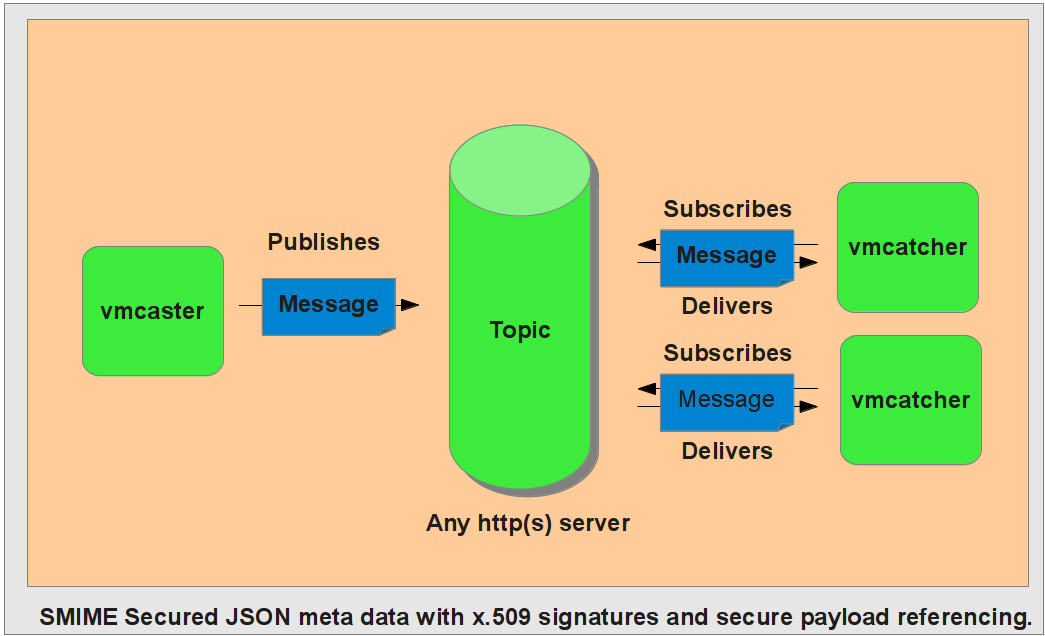
\includegraphics[width=1\textwidth]{vmcaster_vmcatcher.png}
\caption{VMcaster and VMcatcher infrastructure.}
\label{fig:infrastructure}
\end{figure}

\subsection{Publishing image lists}
Publishing images according to the HVWG's proposals is as simple as generating the meta data and signing it with standards SMIME signature routines. No new software is needed for this task. Due to the amount of meta data recommended by the HVWG and the expectation that users may want to add their own additional meta data, it is expected that users will use tools for generating the necessary JSON file.

Image lists use a JSON meta data file signed with SMIME  with a secure hash. However the amount of meta data recommended by the HVWG is burdensome to enter by hand.
 
VMcaster is a simple tool for publishing, managing and updating virtual machines image lists which follows the HVWG image list specifications. It was released after the EGI federated Cloud taskforce started using the HVWG's recommendations. 

All the image lists and metadata created by VMcaster are signed and trusted with a X.509 certificate.
This provides a mechanism by which a virtual image can be checked for validity by any subscriber. Any user can check the image list expiration date, if it was revocated or it has been tampered by a third party.
All images and image lists have an Universal(ly) Unique Identifier (UUID). These UUID's should be globally unique and consequently the UUID should be generated using a UUID generator using suitable seeds. As example for Debian, Redhat and Scientific Linux users can execute the following UUID generator:
\begin{verbatim}
$ uuidgen

dfc470ab-0845-4c3b-bc6a-02f990388a17
\end{verbatim}
We can use the new UUID with VMcaster to create a empty image list:
\begin{verbatim}
$ vmcaster --select-imagelist dfc470ab-0845-4c3b-bc6a-02f990388a17 \
--add-imagelist
\end{verbatim}
This command generates an empty image list in our local \textit{vmcaster.db} database (not published yet) with a few predefined objects. We can query the image list ID to see the current object list.
The database information is shown in JSON format:
\begin{verbatim}
$ vmcaster --select-imagelist dfc470ab-0845-4c3b-bc6a-02f990388a17 \
--show-imagelist
{
    "hv:imagelist": {
        "dc:identifier": "dfc470ab-0845-4c3b-bc6a-02f990388a17"
    }
}
\end{verbatim}
The object \textit{dc:identifier} contains always an UUID and it is included in images or image lists. 
At this moment the image list does not include any relevant information but thanks to VMcaster utility the image list endorser can introduce new objects and information.
The most important objects are: the image title, its description, its endpoint (a valid \textit{url}) and also the endorser unique certificate DN. Only a trusted endorser can modify or update an VMcaster image list to include or remove VM images. 
These values can be included into the internal database running these commands, as example:
\begin{verbatim}
$ vmcaster --select-imagelist <image_list_UUID> \
--key-set-imagelist "dc:title"\ 
--key-value-imagelist "New image list"

$ vmcaster --select-imagelist <image_list_UUID> \ 
--key-set-imagelist "dc:source" --key-value-imagelist "CESGA"

$ vmcaster --select-imagelist <image_list_UUID> \ 
--key-set-imagelist "dc:description"\ 
--key-value-imagelist "My image list for internal users"

$ vmcaster --select-imagelist <image_list_UUID> \ 
--key-set-imagelist "hv:uri" --key-value-imagelist \ 
"http://cloud.cesga.es/files/image.list"

$ vmcaster --select-endorser \ 
"/DC=es/DC=irisgrid/O=cesga/CN=alvarosimon" \
--key-set-endorser "dc:creator" --key-value-endorser "Alvaro Simon"
\end{verbatim}

Endorsers can also import image lists (in JSON or MIME format) to streamline the image list creation. At this moment the endorser can include new images metadata into the new image list catalogue.
Image insertion procedure is similar to image list creation \textit{vmcaster --select-image <UUID> --key-set-image <IMAGE TAG> --key-value-image <VALUE>}.  
The image list endorser only has to generate a new UUID and insert the relevant objects, in this case:
\begin{itemize}
 \item \textit{dc:title}: Image title name
 \item \textit{sl:comments}: It includes image comments (user login and password, software included etc).
 \item \textit{sl:osversion}: The Operating System version as LSB compliant. As example Scientific Linux release 6.4 (Carbon).
 \item \textit{sl:arch}: System architecture (x86\_64, i386 etc).
 \item \textit{sl:os}: Operating System name (Ubuntu, Debian, RedHat..).
 \item \textit{hv:uri}: Image location endpoint. The image must be accesible from this url. As example \url{http://cloud.cesga.es/images/debian-6.0.5-x86_64-base.qcow2}
 \item \textit{hv:format}: VM image format (QCOW2, RAW)
\end{itemize}
All the new images should be assigned to a image list, we can include the same image in different image lists. To add a new image to a specific image list:

\begin{verbatim}
$ vmcaster --select-imagelist <IMAGE_LIST_UUID> \
--imagelist-add-image --select-image <IMAGE_UUID>
\end{verbatim}

VMcaster can be configured to syncronize and upload local images to a specific server endpoint. This mechanism allows to VMcaster users to upload images and image lists to a web server in an automated way.
This information is located into a configuration file (\textit{/etc/vmcaster/vmcaster.cfg}). This mechanism is very useful for Image List endorsers as they can use this configuration file to include several servers to keep the image lists up to date in a short period of time.
\textit{vmcaster.cfg} file uses this schema:
\begin{verbatim}
[SERVER NAME]
server = "myserver.org"
protocol = "scp"
uriMatch = "https://myserver.org/"
uriReplace = "user@myserver.org:/var/www/html/"
\end{verbatim}
In this case VMcaster will use the \url{myserver.org} web page to upload any image or image list. 
\textit{vmcaster.cfg} accepts different communication protocols such scp, GSIdCap~\cite{dcache} or a local transmission. If this configuration file is set, VMcaster will upload images automatically using this command:

\begin{verbatim}
vmcaster --upload-image <local_image_path> \
--select-image <IMAGE_UUID>
\end{verbatim}

VMcaster detects the image size and generates a SHA512 hash for each uploaded image, when this process is complete the updated information is included into the VMcaster database automatically.

At the end the information can be gathered from the local database, as example using JSON format image list:
\begin{verbatim}
{
    "hv:imagelist": {
        "dc:date:created": "2013-03-18T16:52:55Z", 
        "dc:date:expires": "2014-04-15T16:52:55Z", 
        "dc:description": "CESGA image list for internal usage", 
        "dc:identifier": "2204eed5-f37e-45b9-82c6-85697356109c", 
        "dc:source": "CESGA", 
        "dc:title": "CESGA image list", 
        "hv:endorser": {
            "hv:x509": {
                "dc:creator": "Alvaro Simon Garcia", 
                "hv:ca": "/DC=es/DC=irisgrid/CN=IRISGridCA", 
                "hv:dn": "/DC=es/DC=irisgrid/O=cesga/CN=alvarosimon", 
                "hv:email": "asimon@cesga.es"
            }
        }, 
        "hv:images": [
            {
            {
                "hv:image": {
                    "dc:description": "UI-UMD3.0.0", 
                    "dc:identifier":\ 
"9d6b140f-7a08-4f8c-8c25-3564bcb50e33", 
                    "dc:title": "EMI-UI", 
                    "hv:format": "QCOW2", 
                    "hv:hypervisor": "QEMU,KVM",  
                    "hv:uri":\ 
"http://cloud.cesga.es/images/test_ui_image.QCOW2", 
                    "hv:version": "0.0.1", 
                }
            }
        ], 
        "hv:uri": "http://cloud.cesga.es/files/image.list", 
        "hv:version": "2.9"
    }
}
\end{verbatim}
By reading the image list example in JSON format, a future subscriber can identify the available images, the image list creation/expiration dates or the endorser DN.

When the image list is ready and updated the endorser can publish it to all sites included into the \textit{vmcaster.cfg} file. 
The procedure is quite similar to the image uploading, but in this case, the image must be signed by the endorser certificate to validate its authenticity.
VMcaster asks for user certificate password and uploads the image list to its final endpoint, this can be done with a single command:
\begin{verbatim}
$ vmcaster --select-imagelist <IMAGE_LIST_UUID> --upload-imagelist
\end{verbatim}
This procedure allows different image endorsers to distribute and update image catalogs on different endpoints and sites (which is suitable for a federated architecture).
Besides all image lists has endorsed information about endorser certificate public key, image download endpoint, initial global validity, etc. 
That means valid images can be selected, downloaded and instantiated and tested by different resource provides. 
The new images should be verified by the image list endorser but fedcloud resource provides have the final say about its inclusion into their Cloud image repositories. 
Image subscription task is done by VMcatcher utility described in the next section.


\subsection{Subscribing to image lists}
VMcatcher~\cite{vmcatcher} is currently the only HVWG image list subscriber, and only supports JSON meta data and X.509 signatures. Since the Grid community already use the International Grid Trust Federation~\cite{igtf} supporting just x.509 is acceptable for the current stage for the Federated cloud task force so these limitations nave not hindered this investigation. 
It is recommended that future HVWG image list providers support PGP and X.509 signatures.

VMcatcher allows subscription of virtual machine images by UUID so that a resource provider can provide contextualised appliance images from the most recent appliance image. Resource providers can configure their own image lists and select images from an image list, these are then validated in compliance with the HVWG security policies and cached locally. 
VMcatcher does not support any cloud explicitly so further work was needed in this area.

VMcaster can be configured to launch applications on image status change events such as expiry or new images becoming available. The federated Cloud task force has developed such integration handlers for managing Appliance Life cycle management with OpenStack and OpenNebula.

Using this utility users can select and download trusted images.
This utility caches the selected images in a image list, validates the list with X.509 based public key cryptography, and also checks the images SHA512 hashes. 

VMcatcher and VMcaster work in a similar way. They are based upon a local database that stores subscriptions to VM image lists, registered endorsers, and which images belong to which subscriptions. 
This enables images to be selected for subscription. An user can select the desired image from the lists and then set the desired image subscriptions.
Subscribed images can be downloaded, verified and cached. VMcatcher also verifies if the cached images have expired or not. If an image is invalid or it has expired it is moved to an expiry directory.
The image consumer must trust in a endorser, in this case users can include and confirm their trust in a image endorser based on his/her X.509 certificate Distinguished Name (DN).
To include a new trusted endorser:
\begin{verbatim}
$ vmcatcher_endorser --create --endorser_uuid='Alvaro Simon' \
--subject='/DC=es/DC=irisgrid/O=cesga/CN=alvarosimon' \
--issuer='/DC=es/DC=irisgrid/CN=IRISGridCA'
\end{verbatim}
And now the user only has to download the desired image list from the endpoint and import it into a local VMcaster database:
\begin{verbatim}
$ wget http://cloud.cesga.es/files/image.list
$ vmcatcher_subscribe -s file:////`pwd`/image.list
\end{verbatim}
At this point the image user can show and select any image UUID from the new list to be downloaded. 
The image list may vary (image endorse includes new images, revoke old ones, etc), in any case the local image list database should be updated frequently executing the command \textit{vmcatcher\_subscribe -U}.
This command checks the image lists endoint and updates the local database accordingly.
After image selection the images can be downloaded and updated to a local cache running:
\begin{verbatim}
$ vmcatcher_cache
\end{verbatim}

The new downloaded images are stored into \textit{<VMCATCHER\_DIR>\-/cache} directory, meanwhile revoked or expired images are moved to \textit{<VMCATCHER\_DIR>\-/cache\-/expired} directory. 
This mechanism prevents that old or revoked images are used by mistake.  


\section{Image management event handlers}
\label{sect-handlers}
VMcatcher and VMcaster are useful tools to disseminate and keep updated our images but they do not interact with Cloud frameworks directly.
VMcatcher was written in Python and generates pre-defined events that can be received by an asynchronous callback subroutine or event handler.
These pre-defined events can be used by the Cloud frameworks to perform different actions.

Fortunately the Cloud community has developed event handlers to interact with the most popular frameworks like OpenNebula or CloudStack.
OpenNebula event handler~\cite{onevent} was developed by the CESGA team and currently is available from the VMcaster repository. 
The \textit{vmcatcher\_eventHndlExpl\_ON} package provides a new python and cron script which detects VMcatcher events. 
This script detects several VMcatcher event types. In this case OpenNebula handler only waits for a new Expire or Available VMcatcher event.
If VMcatcher raises a \textit{AvailablePostfix} event, this is detected by \textit{vmcatcher\_eventHndlExpl\_ON} event handler and reads the new image attributes such UUID, image name, description and image format.

\begin{figure}
\centering
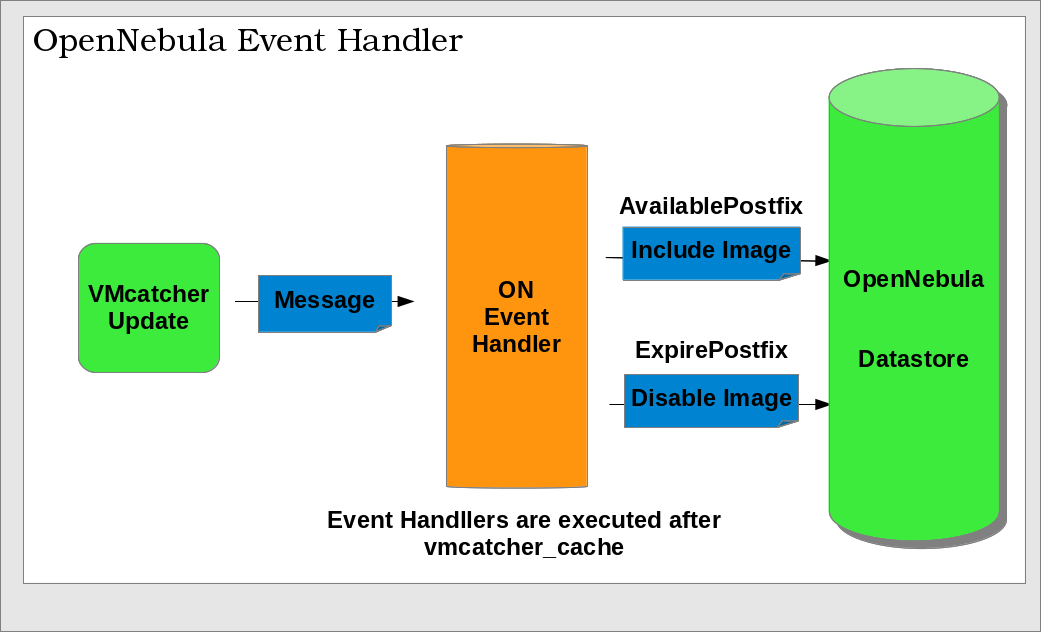
\includegraphics[width=1\textwidth]{ONeventhandler.png}
\caption{OpenNebula event handler.}
\label{fig:onevent}
\end{figure}

If a new image is downloaded (\textit{AvailablePostfix} event), the OpenNebula event handler gets the image information, generates a new OpenNebula template and includes the new image into the local OpenNebula datastore (see figure \ref{fig:onevent}). 
For security reasons, the new images are not public, they are only available for the oneadmin user. The OpenNebula administrator should verify the new image first (checking its contextualisation script, if the image is executed correctly etc).

After this period of time the image status is changed to be available for external users. 
Moreover if VMcatcher detects an image revocation the OpenNebula event handler searches the image UUID from OpenNebula image database and it is set to disable status.
The image is not removed by the event handler, it should be removed by the site administrator from the OpenNebula datastore.

The OpenNebula event handler is not the only available one. OpenStack administrators can also use Glancepush~\cite{glancepush} service to keep their local image catalog updated. 
This service was developed at IN2P3 and it works in a similar way than the OpenNebula event handler. 
In this case Glancepush updates the OpenStack Image Service (Glance) if it detects any image change from VMcatcher tool. 
The new package (\textit{glancepush-vmcatcher}) is available from the IN2P3 ftp server, and it only requires a working glance service and an OpenStack user account to push images into the catalog.

%\section{Use Case: EGI SA2.3 verification image repository}
%\label{sect-usecase}
%This is my text 

\section{Conclusions and Future work}
\label{sect-conclusions}
The management of virtual machine images is a critical task within a federated Cloud architecture. It involves certain safety standards and special scalability and availability and stability patterns.
Taking these requirements into account Fedcloud taks force have chosen VMcaster and VMcatcher utilities to distribute and validate VM images between the resource providers.
Fedcloud resource providers are using a heterogenous Cloud frameworks ecosystem (OpenStack, OpenNebula, WNoDES~\cite{wnodes}, etc). This kind of federated infrastructure requires agnostic tools.
Fortunately as we have explained in this paper, VMcatcher can be used by any Cloud framework to distribute and update images in a transparent way. 
The new image management tools are being successfully used by EGI Fedcloud providers since last year and it will be used in more use cases in the near future.

The greatest potential for the EGI-federatred cloud task force is to simplify the management of IaaS systems with respect to the native IaaS Clouds own API's. 
However Cloud implementation neutrality increases the Interoperability challenges. 
The HVWG propsal is esentially federated with a distributed system, no single point of failure or single service in control, and with a policy that was agreed by the mebers of the HVWG as a secure best practice.
The use of a simple signed lists of endorsed Appliances in these proposals is equally applicable to all PKI infrastructures supported by SMIME. 


We believe that the HVWG proposal to manage Appliance Lifecycle, with signed messages listing Appliances that are valid and expressive enough for federating appliances. 
Appliance image distribution and management is typically I/O bound and so asynchronous in nature signed aplliance images list provide a simple and clear way of managing appliance images that can be audited by resource providers. 
We found the clear definition of valid and invalid/expired images, and the distributed nature of Appliance lists a natural fit to a federated cloud and worth testing.

Having tested the use of HVWG proposed image distribution system, with the tools VMcaster and VMcatcher, and having developed event handlers for vmcatcher, the Federated Cloud Task force have proved that this approach is a distributed system for image distribution, for both Open Stack and Open Nebuala resource providers. 
The Fedcloud task force have validated VMcaster and VMcatcher utilities as production grade implementation, and will continue to be uses them to distribute and validate VM images.

EGI Fedcloud task force is committed to support these new image managements tools in the future and the developmnet work is still on going within the project. 
GRNET partner is developing a new Virtual Appliance Marketplace based on EGI Applications Database (EGI AppDB), a project service which stores and provides to the public information about Grid software solutions for scientists and programmers.
This service was extended to create a Virtual Appliance Marketplace tp bring a new category of software entries or virtual appliances, which are virtual machine images designed to run on a virtualization platform.
AppDB's Virtual Appliance Marketplace was integrated with the existing HVWG VMCaster/VMCatcher framework.
EGI Marketpalce uses VMcatcher to download and update the new images included into EGI Image list and provides this list to Fedcloud users.  
The basic image management features were embedded in the Marketplace, such as creating, publishing, enabling/disabling, and archiving or deleting Virtual Appliances or VM image versions.
Besides a friendly site can include its own image list to be published by the Marketplace (see figure \ref{fig:egimodel}). 
This image management model is still under development and testing but it will available in production to be used by EGI users in the next months.

\begin{figure}
\centering
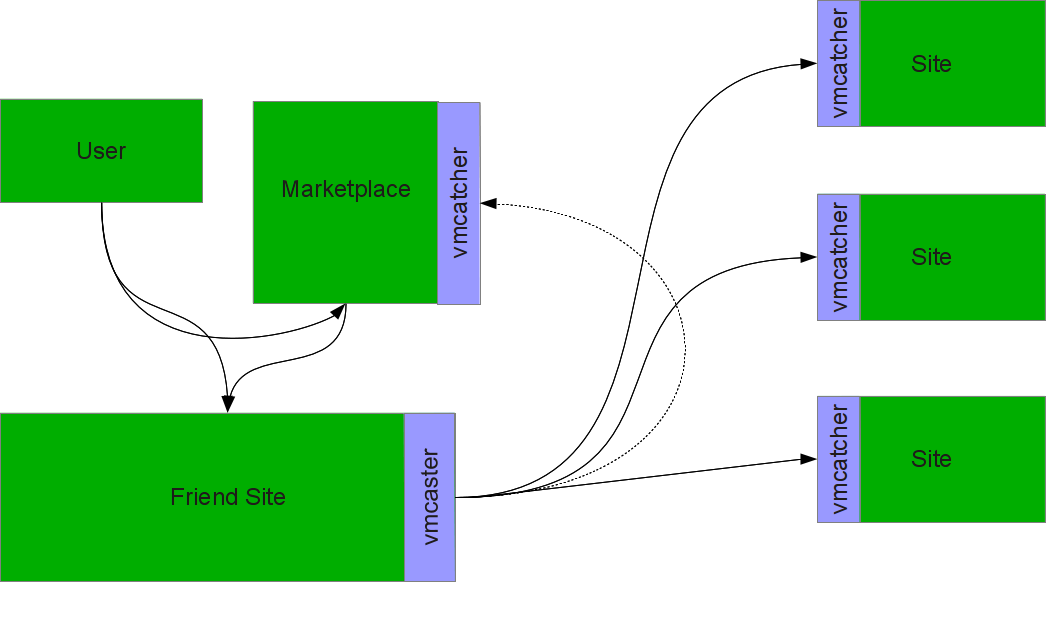
\includegraphics[width=1\textwidth]{egi_model.png}
\caption{EGI Fedcloud Image Management model}
\label{fig:egimodel}
\end{figure}


\section{Acknowledgements}
\label{sect-acknowledgements}
This work is partially funded by the  EGI-InSPIRE (European Grid Initiative: Integrated Sustainable
Pan-European Infrastructure for Researchers in Europe) is a project co-funded by the European Commission 
(contract number INFSO-RI-261323) as an Integrated Infrastructure Initiative within the 7th Framework 
Programme. EGI-InSPIRE began in May 2010 and will run for 4 years. Full information is available at:
\url{http://www.egi.eu/}.


\begin{thebibliography}{99}

\bibitem{Dillon2010}
Dillon, T. et al.: Cloud Computing: Issues and Challenges.
Advanced Information Networking and Applications (AINA), 2010 24th IEEE International Conference, pp.~27--33

\bibitem{Hoffa2008}
Hoffa, C. et al.: On the Use of Cloud Computing for Scientific Workflows.
eScience, 2008. eScience '08. IEEE Fourth International Conference, pp. ~640--645

\bibitem{Lagar-Cavilla2009}
Lagar-Cavilla: SnowFlock: rapid virtual machine cloning for cloud computing.
Proceedings of the 4th ACM European conference on Computer systems, EuroSys 2009, pp.~1--12

\bibitem{Xi2012} 
Chunxiao, L. et al.: A Trusted Virtual Machine in an Untrusted Management Environment.
Services Computing, IEEE Transactions, 
Vol.~5, 2012, No.~4, pp.~472--483

\bibitem{Django2013}
Armstrong, D. et al.: Runtime Virtual Machine Recontextualization for Clouds.
Lecture Notes in Computer Science, Euro-Par 2012: Parallel Processing Workshops, 
Vol.~7640, pp.~567--576

\bibitem{Laszewski2012} 
Laszewski, V. et al.: Comparison of Multiple Cloud Frameworks
Cloud Computing (CLOUD), 2012 IEEE 5th International Conference, pp.~734--741

\bibitem{Diaz2012} 
Diaz, J. et al.: Abstract Image Management and Universal Image Registration for Cloud and HPC Infrastructures,
Cloud Computing (CLOUD), 2012 IEEE 5th International Conference, pp.~463--470

\bibitem{Maurer2013}
Maurer, M. et al.: Adaptive resource configuration for Cloud infrastructure management.
Future Generation Computer Systems,
Vol.~29, 2013, No.~2, pp.~472--487

\bibitem{Schwarzkopf2012}
Schwarzkopf, R. et al.: Increasing virtual machine security in cloud environments.
Journal of Cloud Computing,
Vol.~1, 2012, No.~1, pp.~1-12

\bibitem{Zhao2012} 
Yong, Z. et al.: Designing and Deploying a Scientific Computing Cloud Platform.
Grid Computing (GRID), 2012 ACM/IEEE 13th International Conference, pp.~104--113

\bibitem{Goasguen2012}
Goasguen, S. et al.: Lxcloud : a prototype for an internal cloud in HEP. Experiences and lessons learned.
Journal of Physics: Conference Series,
Vol.~396, 2012, No.~3

\bibitem{Xiaolong2012}
Wen, X. et al.: Comparison of open-source cloud management platforms: OpenStack and OpenNebula.
Fuzzy Systems and Knowledge Discovery (FSKD), 2012 9th International Conference, pp.~2457--2461


\bibitem{vmcaster}
VMcaster VM image publication tool. \\
\texttt{https://github.com/hepix-virtualisation/vmcaster}, 2013 \\
\textit{Last visit on November 2013}

\bibitem{vmcatcher}
VMcatcher image subscription tool. \\
\texttt{https://github.com/hepix-virtualisation/vmcatcher}, 2013 \\
\textit{Last visit on November 2013}

\bibitem{hepix}
Tony Cass: The HEPiX Virtualisation Working Group: Towards a Grid of Clouds.
Journal of Physics: Conference Series,
Vol.~396, 2012, No.~3

\bibitem{dcache}
Mathias De Riese: The dCache Book. \\
\texttt{http://www.dcache.org/manuals/Book/}, 2013 \\
\textit{Last visit on November 2013}

\bibitem{onevent}
OpenNebula event handler. \\
\texttt{https://github.com/grid-admin/vmcatcher\_eventHndlExpl\_ON}, 2013 \\
\textit{Last visit on November 2013}

\bibitem{glancepush}
OpenStack Glancepush service. \\
\texttt{https://github.com/EGI-FCTF/glancepush/wiki}, 2013 \\
\textit{Last visit on November 2013}

\bibitem{wnodes}
Salomoni, D. et al.: WNoDeS, a tool for integrated Grid and Cloud access and computing farm virtualization.
Journal of Physics: Conference Series,
Vol.~331, 2011

\bibitem{gridcloud}
Zhang, S. et al.: The comparison between cloud computing and grid computing.
Computer Application and System Modeling (ICCASM),
Vol.~11, 2010, pp.~72--75.

\bibitem{igtf}
The International Grid Trust Federation. \\
\texttt{http://www.igtf.net/}\\
\textit{Last visit on November 2013}

\bibitem{appdb}
EGI Applications Database. \\
\texttt{http://appdb.egi.eu/} \\
\textit{Last visit on November 2013}

\end{thebibliography}


%%\bio{}\'Alvaro ,Sim\'on\\ . \dots




\label{lastpage}
\end{document}
